\documentclass{article}

% if you need to pass options to natbib, use, e.g.:
% \PassOptionsToPackage{numbers, compress}{natbib}
% before loading nips_2016
%
% to avoid loading the natbib package, add option nonatbib:
% \usepackage[nonatbib]{nips_2016}

% \usepackage{nips_2016}

% to compile a camera-ready version, add the [final] option, e.g.:
\usepackage[final]{nips_2016}

\usepackage[utf8]{inputenc} % allow utf-8 input
\usepackage[T1]{fontenc}    % use 8-bit T1 fonts
\usepackage{hyperref}       % hyperlinks
\usepackage{url}            % simple URL typesetting
\usepackage{booktabs}       % professional-quality tables
\usepackage{amsfonts}       % blackboard math symbols
\usepackage{nicefrac}       % compact symbols for 1/2, etc.
\usepackage{microtype}      % microtypography

\usepackage{amsmath}	% for \begin{align}
\usepackage{graphicx}	% for \includegraphics{filename}

\newcommand{\bb}[1]{\boldsymbol{#1}}

\title{Adversarial Zero-Shot Learning}

% The \author macro works with any number of authors. There are two
% commands used to separate the names and addresses of multiple
% authors: \And and \AND.
%
% Using \And between authors leaves it to LaTeX to determine where to
% break the lines. Using \AND forces a line break at that point. So,
% if LaTeX puts 3 of 4 authors names on the first line, and the last
% on the second line, try using \AND instead of \And before the third
% author name.

\author{
	Shihui Li, Yu-Hsiang Lin, Kangyan Zhou
		%\thanks{Use footnote for providing further information about author (webpage, alternative address)---\emph{not} for acknowledging funding agencies.}
		\\
	Language Technologies Institute\\
	Carnegie Mellon University\\
	Pittsburgh, PA 15213 \\
	\texttt{\{shihuil,yuhsianl,kangyanz\}@andrew.cmu.edu} \\
	%% examples of more authors
	%% \And
	%% Coauthor \\
	%% Affiliation \\
	%% Address \\
	%% \texttt{email} \\
	%% \And
	%% Coauthor \\
	%% Affiliation \\
	%% Address \\
	%% \texttt{email} \\
}

\begin{document}
% \nipsfinalcopy is no longer used

\maketitle

%\begin{abstract}

%	This is a 4-page draft.

%\end{abstract}



% ----------------------------------------------------
% ----------------------------------------------------

\section{Introduction}

Zero-shot learning has been a hot research topic in the field of image classification. It simulates how people learn things: when people see an unfamiliar object, we would like to use our existing knowledge and try to evaluate the new object. Ideally, a large-scale image classification system should be able to recognize novel categories based on its previous training experience. One of the main challenges for object recognition is the lack of sufficient annotations for all possible concepts. This problem becomes even more severe when we target at the task of fine-grained classification because the annotation is more expensive and the number of fine-grained classes is huge. Realizing this limitation, researchers resort to additional information, for example attributes or text, to solve this problem.  

On the other hand, autoencoder has shown its great express power to present complicate distributions such human faces, natural sceneries and natural language. Autoencoder is able to convert complicated real world data distributions, e.g. text features, to very well-formed low dimension. Many studies have shown that after applying autoencoder techniques, the learned latent feature space often has clear semantic meanings. For example, in \cite{makhzani2015adversarial}, all the digits can be well embedded into a low-dimensional manifold such that similar digits will have smaller distance within that manifold.

 \par 

The fundamental problem of zero-shot learning is to extract semantically meaningful feature embeddings that could bridge the gap between similar image/text features and fine-grained classes. Autoencoder becomes an ideal option for this task because it can automatically learn important features. In \cite{kodirov2017semantic}, they present a novel solution to zero-shot learning based on learning a Semantic AutoEncoder(SAE). Taking the encoder-decoder paradigm, an encoder aims to project a visual feature vector into the semantic space as in the existing zero-learning shot models and the decoder should be able to reconstruct the original visual feature. Their results show that under this framework, the learned projection function from the seen classes is able to generalize better to the new unseen classes. One shortcoming of this model is that the encoder tends to learn similar features across multiple classes, which is disappointing for the task of fine-grained classification. 

Inspired by these models, we propose an Adversarial Semantic AutoEncoder(ASAE). In our model, we have an encoder that projects a visual feature vector into the semantic space and a decoder that decodes and reconstructs the original visual features. Besides, we incorporates a discriminator as in \cite{makhzani2015adversarial} to ensure that generating from any part of prior space results in meaningful samples. Two types of discriminators will be discussed in this project, one is independent from semantic space and the other is dependent from semantic space. 

% In this project we plan to explore how to develop an effective transfer learning algorithm, with focus on zero-shot learning and its combination with several popular deep learning methods, such as convolutional neural network, attention models, and Adversarial training, to detect unseen objects only with text description. \\
% Zero-shot learning consists in learning how to recognize new concepts by just having a description of them. State-of-the-art methods for zero-shot recognition formulate learning as a embedding problem of images and side information like text \cite{Elhoseiny2013}. We propose a model that can classify unseen categories from their textual description. Inspired by the fact that there is little supervision on text data, certain noise-cancelling techniques could be applied to improve the performance of our model.\\




% ----------------------------------------------------
% --------------------------------------------------


\section{Related Works}    
Considering that fine-grained categories might share some common knowledge, a common approach is to seek for an intermediate semantic representation that could connect seen and unseen classes. Human specified attributes are first explored to represent the discriminative properties shared among both seen and unseen categories in zero-shot learning\cite{torresani2010efficient, lampert2009learning}. One limitation of this method is that the creation of attributes still relies on human labors, making it difficult to scale up to meet large scale needs. \par 

%Other forms of semantic representations have been explored since then. \cite{torresani2010efficient} employs the idea of using object detectors as the basic representations of images and the semantic concept is trained by using the entire image. \cite{mensink2014costa} attempts to capture the semantic relevance of two concepts by the co-occurrence of words.  In \cite{mensink2014costa, romera2015embarrassingly}, the authors assume that the classifier for an unseen class can be presented as a linear combination of seen class classifiers.

Apart from handcrafting attributes, another scheme is to directly use the online textual document as the additional information source. \cite{Elhoseiny2013} is one of the first works to use Wiki documents as text attributes. \cite{Ba_2015_ICCV} proposed a model that changes both the ways of extracting features from images and text domains. More specifically, the image features are extracted from the activation layer of a convolutional neural network(CNN), and then go through a linear projection layer to reduce dimensions. The input text, e.g. Wikipedia articles, is first converted to one-hot encodings of the words with their tf-idf scores, which can be viewed as attributes, and then fed into a multi-layer perceptron (MLP) to generate a deep representation, with the same dimension as the final image feature, and unique for each class. The final prediction is obtained by the dot product of the two generated features. Instead of learning an embedding space for each modalities, \cite{frome2013devise} learns joint image-word embeddings so as to embedding images and sentences into a common space.\\
	
	Another line of research is to improve the quality of the classification procedure. \cite{hariharan2012efficient} firstly proposed a SVM based classifier which takes the linear projection of both source and target domain data as the combined input. More recent works jointly project the class into an embedding space, and try to compute a compatability function $F(x, y)$ that tries to predict whether the image feature x is compatible with the embedded class feature y. Here each class is represented as a vector that contains the relevance scores of the class and a set of predefined attributes.  In \cite{akata2013label}, $F(x, y)$ takes a linear form as $F(x, y) = xWy$. \cite{xian2016latent} takes this idea one step further, where a set of $W_i$ is available for the the compatibility function $F(x, y)$, and the final prediction will choose the $W$ that can produce the highest score. This $W_i$ can be shared across different labels.  The method is called as latent embedding, since it learns a latent embedding space explicitly based on clustering. \cite{zhang2016zero} proposes a framework that generalizes deep learning embedding, label embedding, and latent embedding. \\ 
    
    Recently deep encoder-decoder has become popular for a variety of multi-modal problems. In \cite{kiros2014unifying}, they introduce an encoder-decoder pipeline that learns a multimodal joint embedding space with images and text and a novel language model for decoding distributed representations of the text semantic space. Their pipeline effectively unifies joint image-text embedding models with multimodal neural language models. \cite{kodirov2017semantic} takes a step further in multimodal model under the autoencoder paradigm. They proposed a novel zero-shot learning model based on a semantic autoencoder that uses a fast linear projection function and introduce an additional reconstruction objective function for learning a more generalisable projection function. \\ 


% 	In \cite{Elhoseiny2013}, during training, they learn the domain transfer function, $W$, from text domain to vision domain (in addition to feature extraction from text and image data). They use the approach from \cite{Kulis2011}. There is a measure of how much two feature vectors ($\bb{t}$ from text domain and $\bb{x}$ from vision domain) are similar to each other, based on $\bb{t}^{\top} W \bb{x}$. The training objective is basically that: (1) if $\bb{t}$ and $\bb{x}$ belong to the same class, their similarity should be more than a positive threshold (a margin), and (2) if $\bb{t}$ and $\bb{x}$ belong to the different classes, their similarity should be less than a negative threshold (a margin). It is trained with some regularization. (If the objective function is a direct/simple function of $\bb{t}^{\top} W \bb{x}$, it is non-convex for $\bb{t}$ and $\bb{x}$. That might be the reason that in \cite{Kulis2011} they use a more sophisticated formulation.)
	
% 	In fact, in \cite{Elhoseiny2013} during training they also need to learn the weight vectors $\bb{w}_i$, $i = 1, \dots, N_{sc}$ for ``seen classes'', but it seems that they do not describe how they learn these classifiers.
	
% 	They said that they ``learn'' the weight predictor (or the ``classifier regressor'') during training, but from their formulation it seems that as long as you have $\bb{w}_i$, then what the predictor does is that, given a new text vector $\bb{t}$, use $\bb{w}_i$ and Gaussian kernels (presumably with some fixed hyperparameters?) to compute (through an optimization problem) the predicted weight vector. So there doesn't seem to be any model parameters to learn here, but only works to do during inference time.
	
% 	During test time (inference), they give a clear constrained optimization problem to solve. What they try to optimize (in order to obtain the predicted weight vector $\bb{w}$ for an unseen-class text data $\bb{t}$) is basically:
% 		\begin{enumerate}
% 			\item Maximizing the similarity between $\bb{w}$ and $\bb{t}$ with respect to the domain transfer function $W$ (note that $W$ was trained using image feature $\bb{x}$ but here it is applied to weight vector $\bb{w}$ in image domain).
% 			\item Maximizing the log probability of having this $\bb{w}$ given $\bb{t}$ with respect to the weight predictor (and a given Gaussian prior).
% 			\item Minimizing the margin (well, it seems to be unbounded if you try to maximize the margin) of correctly labeling the seen classes all into negative side (they do not belong to the new class).
% 			\item Minimize the L2 regularizor.
% 		\end{enumerate}
% 		Their constraints are that all the seen images are classified as negative with some margin (done the slack variables, the margin, which are minimized).
	
	



% ----------------------------------------------------
% ----------------------------------------------------

% ----------------------------------------------------

% \subsection{Adversarial autoencoder}

% 	The adversarial autoencoder is a mixture of an autoencoder and a generative adversarial network. The input image $\bb{x}$ is encoded into $\bb{h}$ through encoder function $\bb{h} = f_{enc}(\bb{x})$. The reconstruction is performed by the conjugate decoder function $\tilde{\bb{x}} = f_{dec}(\bb{h})$. The autoencoder is trained to reconstruct the input image by minimizing the cross entropy loss,
% 		\begin{align}
% 			\textrm{loss} = -\bb{x}^{\top} \log \tilde{\bb{x}}.
% 		\end{align}
	
% 	The encoder also serves as the generator of the adversarial network, which generates negative samples with aggregated posterior distribution $q(\bb{h})$ that comes from the encoding distribution $q(\bb{h} | \bb{x})$ and the data distribution $p_d(\bb{x})$,
% 		\begin{align}
% 			q(\bb{h}) = \int q(\bb{h} | \bb{x}) p_d(\bb{x}) d \bb{x}.
% 		\end{align}
	
% 	A discriminator $D(\bb{z})$ gives the probability that $\bb{z}$ is a positive sample generated from a given and fixed prior distribution $r(\bb{z})$. The generator (the encoder) and discriminator are then jointly trained according to
% 		\begin{align}
% 			\min_{f_{enc}} \max_D \left\{ E_{\bb{z} \sim r(\bb{z})}[ \log D(\bb{z}) ] + E_{\bb{x} \sim p_d(\bb{x})}[ \log( 1 - D(f_{enc}(\bb{x})) ) ] \right\}.
% 		\end{align}
% 		That is, the generator (the encoder) is trained to generate samples mimicing the samples produced by the prior (such that the discriminator tends to classify it as positive samples from prior), and the discriminator is trained to classify the samples from prior as positive and those from generator as negative. The optimal solution is that the generator generates samples exactly according to the prior distribution (i.e.~$q(\bb{h}) \propto r(\bb{z})$), and the discriminator classifies samples from either the prior or the generator as positive samples with equal probabilities (e.g.~$D(\bb{z}) = D(f_{enc}(\bb{x})) = 1/2$).



% ----------------------------------------------------
% ----------------------------------------------------

\section{Zero-shot learning task}

	We aim to solve the zero-shot learning problem of classifying images of unseen classes. Given the training images $\bb{x}^c$ and their corresponding text description documents $\bb{t}^c$ for $N_s$ seen classes $c$, we learn the semantic encodings $\bb{h}^c$ of the images. The learning goal is to learn the encodings $\bb{h}^c$ for a class that are close to their corresponding text document representation for this class. The encodings $\bb{h}^{c_1}$ and $\bb{h}^{c_2}$ from two different classes should bear some separable differences.
	
	During the test time, we are given images $\bb{x}^c$ of $N_{us}$ unseen classes $c$ and also their text description documents $\bb{t}^c$, but without the prior knowledge of the correspondence between the images and the text documents. Our task is to predict the corresponding text document given an image.



% ----------------------------------------------------
% ----------------------------------------------------

\section{Adversarial autoencoder for zero-shot learning}

	We propose two architectures that make use of adversarial autoencoders for the zero-shot learning tasks. In one of them we draw positive samples from the prior that is a Gaussian noise, and explicitly require the encoding $\bb{h}^c$ to match the text representation $\bb{t}^c$. In this case, the prior serves as a regularizer, which is presented in Sec.~\ref{subsec:NoisePrior}. In the other of them, we directly use the text representation as positive samples drawn from some distribution that describes a class of data, and the code is trained by the adversarial net to match the text representation. In this case, the prior guides the generator (the encoder) to learn the code that is close to the semantic representation of text, which is presented in Sec.~\ref{subsec:TextPrior}.



% ----------------------------------------------------

\subsection{Prior as regularizer}
\label{subsec:NoisePrior}
	
	The architecture in Figure \ref{fig:NoisePrior} has an autoencoder that learns the encoding $\bb{h}^c$ of the input images $\bb{x}^c$ belonging to a class $c$. The code $\bb{h}^c$ is explicitly required to match the text representation $\bb{t}^c$ of that class, as well as regularized by the prior in the adversarial net. The learning task can be expressed as the optimization problem,
	\begin{align}
		\min_{G} \max_D E_{\bb{z} \sim r(\bb{z})}\left[\; \log D(\bb{z}) \;\right] + E_{\bb{x} \sim p_d(\bb{x})}\left[\; \log( 1 - D(G(\bb{x})) ) + || G(\bb{x}) - \bb{t} ||_2^2 \;\right].
	\end{align}
	
	Similar architecture has been proposed in \cite{kodirov2017semantic}, in which the explicit matching to the text representation was used to learn the semantic autoencoder for the image input. The difference in our architecture is that we use a adversarial net to regularize the matching to the text representation.
	

% ---------------------------------------------------------

\begin{figure}[!htb]
\centering
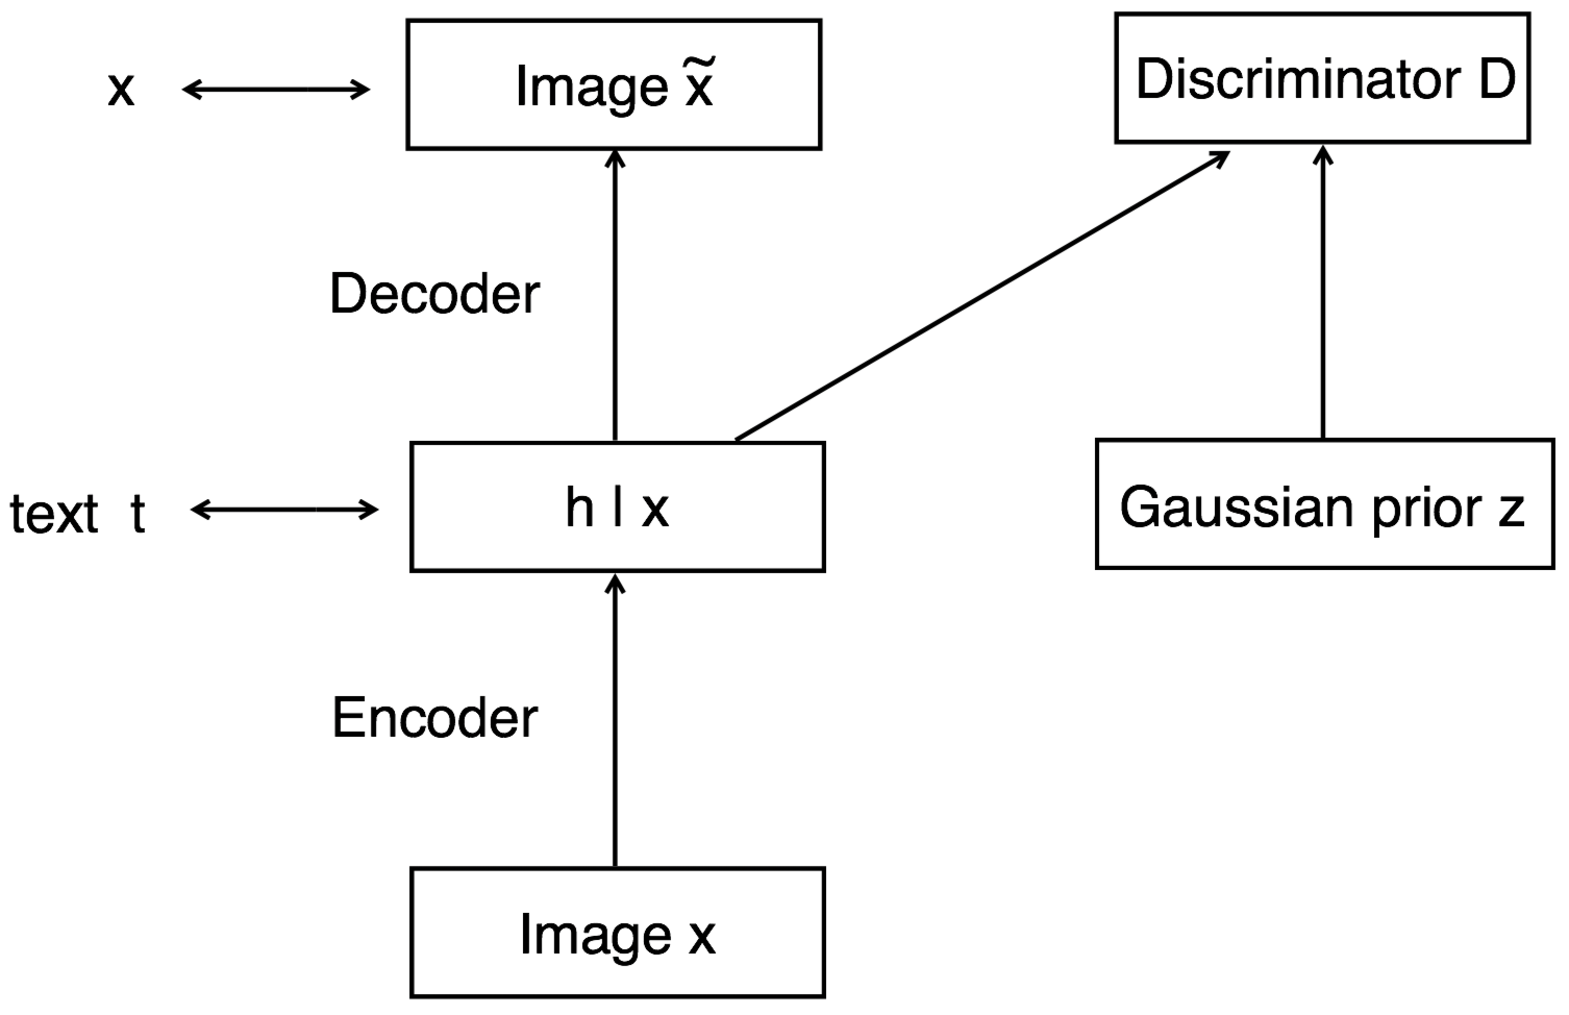
\includegraphics[width = 10 cm]{figNoisePrior}
\caption{Adversarial autoencoder with noise prior and explicit matching to the text representation.}
\label{fig:NoisePrior}
\end{figure}

% ---------------------------------------------------------
% ---------------------------------------------------------

\begin{figure}[!htb]
\centering
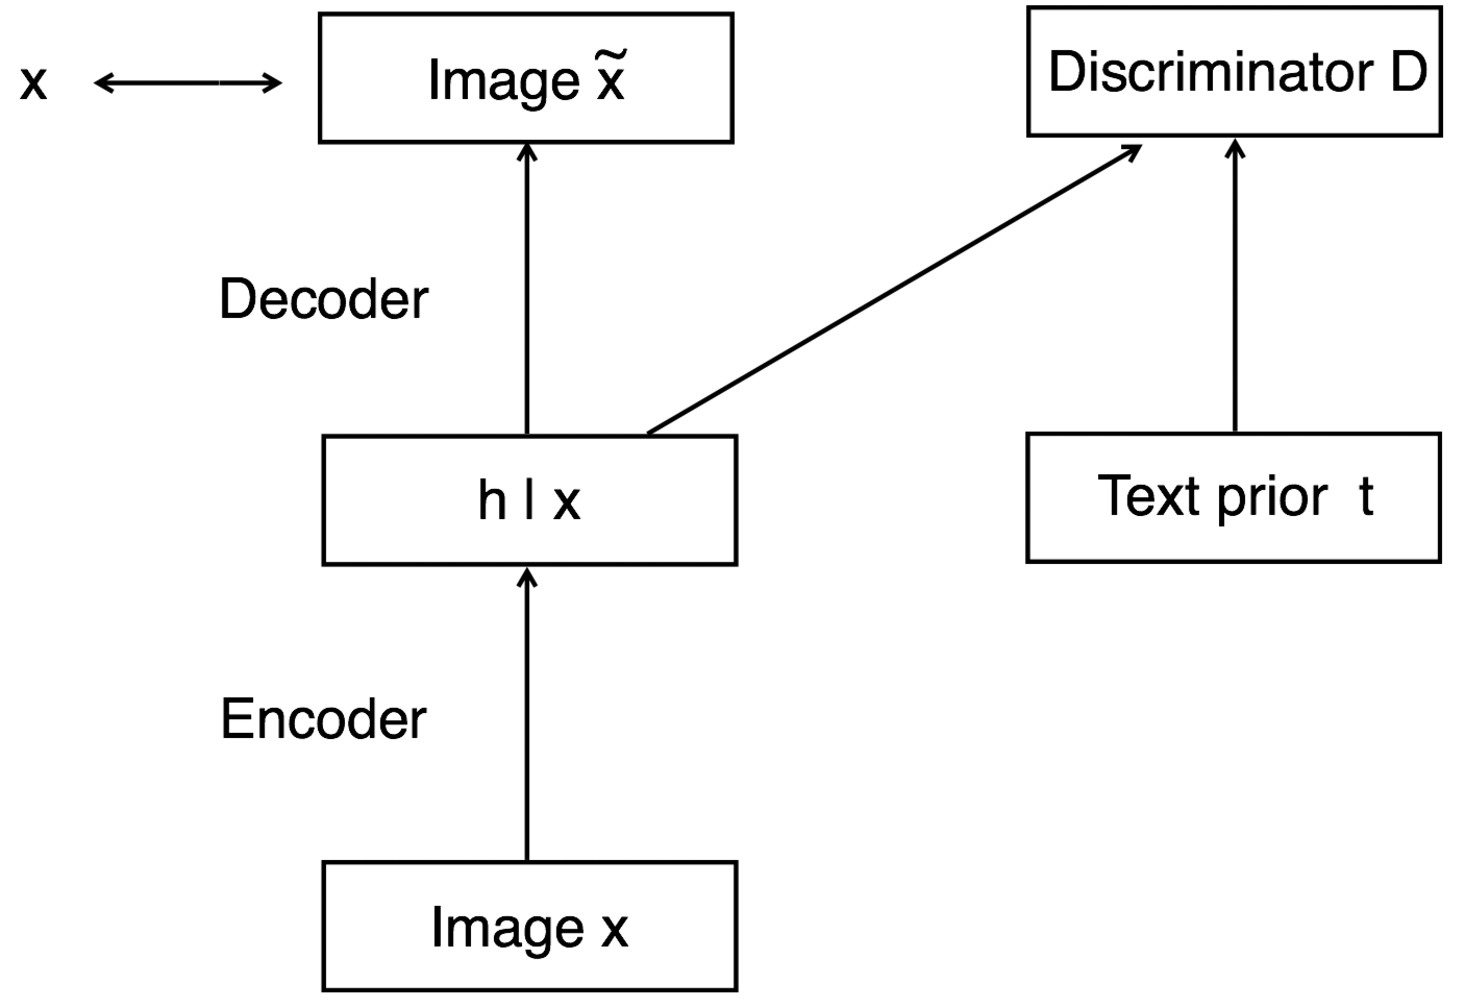
\includegraphics[width = 10 cm]{figTextPrior}
\caption{Adversarial autoencoder with text representations as positive samples drawn from some underlying prior.}
\label{fig:TextPrior}
\end{figure}

% ---------------------------------------------------------





% ----------------------------------------------------

\subsection{Prior as guide}
\label{subsec:TextPrior}
	
	In Figure \ref{fig:TextPrior} we show the adversarial autoencoder that takes the text representation $\bb{t}^c$ as the positive sample drawn from some underlying prior dictating the distribution of the text representation of a class. In this architecture, the code is driven to match the text representation through the adversarial net itself. The optimization problem for this learning scheme is of the same form of the standard adversarial autoencoder,
	\begin{align}
		\min_{G} \max_D E_{\bb{t} \sim r(\bb{t})}\left[\; \log D(\bb{t}) \;\right] + E_{\bb{x} \sim p_d(\bb{x})}\left[\; \log( 1 - D(G(\bb{x})) ) \;\right],
	\end{align}
	except that the prior serves as a guide to match the text distribution rather than as a regularizer that drives the code to a Gaussian noise.










%	We propose to generalize this basic structure to fulfill the zero-shot learning task. In addition to the basic structure of the adversarial autoencoder, we include a domain transfer function $T$. Given the code $\bb{h}^c$ of an image $\bb{x}^c$ coming from a class $c$, the transfer function transforms $\bb{h}^c$ into its corresponding text-domain feature $\bb{\tau}^c = T(\bb{h}^c) = T(f_{enc}(\bb{x}^c))$. We denote the distribution of $\bb{\tau}^c$ as $\bb{\tau}^c \sim s(\bb{\tau}^c | \bb{h}^c, T)$, and the distribution of the actual text in this class as $\bb{t}^c \sim u^c(\bb{t}^c)$. Then, during training, we learn the domain transfer function $T$ such that $s(\bb{\tau}^c | \bb{h}^c, T) \rightarrow u^c(\bb{t}^c)$; that is, the encoded-then-transformed $\bb{\tau}^c$ is similar to $\bb{t}^c$.
	
% 	We propose a novel architecture that jointly learn the the encoding function $f_{enc}$ and the domain transfer function $T$ simultaneously. We adopt the paradigm of the adversarial autoencoder, but instead of using the encoder as the generator, the generator here is the hierarchical structure consisting of the encoder and the domain transfer function, which generates (negative) samples from the distribution $s(\bb{\tau}^c | \bb{h}^c, T)$. The discriminator is trained to classify the actual text $\bb{t}^c$ generated from $u^c(\bb{t}^c)$ (the prior) as positive sample, and the text feature $\bb{\tau}^c$ transferred from the image according to the distribution $s(\bb{\tau}^c | \bb{h}^c, T)$ (that is, $\bb{\tau}^c$ generated by the generator) as negative sample. Note that each class $c$ has its own distinct prior $u^c$. The encoder is in the mean time trained with the decoder to minimize the reconstruction error.
	
% 	During the test time of the zero-shot learning, an unseen test image $\bb{x}$ is given. We feed it into the encoder and the domain transfer function to obtain the text feature $\bb{\tau}$. Then, by computing its similarities to each of the unseen-class actual texts $\bb{t}^1, \bb{t}^2, \dots$, we take the most similar class as the class prediction for this image.
	
% % \noindent\rule{\textwidth}{0.4pt}



% % ----------------------------------------------------

% \subsection{Another possible learning scheme}
	
% 	We consider train the network in two stages: a pre-training to obtain the prior, and then a training of adversarial autoencoder using the pre-trained prior.
	
% 	In the first stage, we learn the domain transfer function, the matrix $W$. (Do we need to use the decoder part of the autoencoder here?) Method: For images $\bb{x}^c_i$ belonging to class $c$, and a text $\bb{t}^c$ in this class, we jointly learn an encoder $W_{enc}$, such that
% 		\begin{align}
% 			\min_{W_{enc}, W} || \bb{h}^c - W \bb{t}^c ||_2^2,
% 		\end{align}
% 		where
% 		\begin{align}
% 			\bb{h}^c = \sigma( W_{enc} \bb{x}^c ).
% 		\end{align}
% 		If we also use decoder part, it will be
% 		\begin{align}
% 			\min_{W_{enc}, W} \alpha || \bb{h}^c - W \bb{t}^c ||_2^2 + \beta [ -(\bb{x}^c)^{\top} \log ( W_{enc}^{\top} \bb{h}^c ) ].
% 		\end{align}

% 	In the second stage, we train the adversarial autoencoder with
% 		\begin{enumerate}
% 			\item $W_{enc}$ initialized by the pre-trained $W_{enc}$ in first stage. It serves as the generator of the adversarial network.
% 			%
% 			\item A class-wise prior
% 				\begin{align}
% 					p^c(\bb{h}^c) = \mathcal{N}( W \bb{t}^c, ( \sigma^{(c)} )^2 I ).
% 				\end{align}
% 		\end{enumerate}
% 		The goal in this stage is to learn (fine tune) the autoencoder $W_{enc}$,
% 		\begin{align}
% 			\min_{W_{enc}} [ -(\bb{x}^c)^{\top} \log ( W_{enc}^{\top} \bb{h}^c ) ],
% 		\end{align}
% 		with the class-wise prior.

% 	In predict time, for a test image $\bb{x}$, compute its code $\bb{h} = \sigma(W_{enc} \bb{x})$. Then predict its belonging text $\bb{t}^*$ among the candidate (unseen-class text) $\{ \bb{t}^1, \bb{t}^2, \dots \}$ by computing $\{ || \bb{h} - W \bb{t}^1 ||_2^2, || \bb{h} - W \bb{t}^2 ||_2^2, \dots \}$ and select the $\bb{t}^c$ of the minimum one as the $\bb{t}^*$.





\section{Dataset Description and Baseline Models}

The dataset we want to use for this project is the Caltech-UCSD Birds 200-2011 data\cite{wah2011caltech}. There are 200 categories of birds. The number of images is 11,788, and the image dimension is 500 $\times$ [300--500] $\times$ 3. Each class consists of between 40 and 80 images. 

Here we also list the baseline models we want to compare out result with. They are Semantic Autoencoder(SAE)\cite{kodirov2017semantic}, Joint Latent Semantic Embedding(JLSE)\cite{zhang2016zero}, and Synthesized classifiers(Sync)\cite{changpinyo2016synthesized}. According to \cite{kodirov2017semantic}, the performance of the baseline models are reported as follows:
\begin{table}[!htb]
 \centering
 \begin{tabular}{|l|l|}
  \hline
  Model & Results \\
  \hline
  SAE\cite{kodirov2017semantic} & 61.4 \\
  \hline
  JLSE\cite{zhang2016zero} & 41.8 \\
  \hline
  Sync\cite{changpinyo2016synthesized} & 54.4 \\
  \bottomrule
 \end{tabular}
 \caption{Performance of baseline models.}
\end{table}






% ----------------------------------------------------
% ----------------------------------------------------

%\section{Data}

%	We use two datasets: The Caltech-UCSD Birds 200 (2010) dataset \cite{Welinder2010}, and the Oxford VGG 102 category flower dataset \cite{Nilsback2008}. The Birds dataset has class number 200, feature dimension 500 $\times$ [300--500] $\times$ 3, and the size of the dataset is 6033. The bird images belonging to 200 species. Each class consists of between 20 and 40 images, with total of 6033 color images in jpeg format.
	
%	The Oxford VGG 102 category flower dataset has class number 102, feature dimension [500--600] $\times$ 500 $\times$ 3, and the size of the dataset is 8189. The flower images belonging to 102 categories. Each class consists of between 40 and 258 images, with total of 8189 color images in jpeg format.






% ----------------------------------------------------
% ----------------------------------------------------

%\section{Discussion}

% 	The architecture proposed in this work can also be applied to image generation from text. By applying the inverse domain transfer function to a given text, $T^{-1}(\bb{t})$ can be taken as the code $\bb{h}$, which can then be fed into the decoder to obtain the image $\bb{x}$.




% ----------------------------------------------------
% ----------------------------------------------------

%\subsubsection*{Acknowledgments}

%Use unnumbered third level headings for the acknowledgments. All acknowledgments go at the end of the paper. Do not include acknowledgments in the anonymized submission, only in the final paper.



% ----------------------------------------------------
% ----------------------------------------------------

\bibliographystyle{plain}
\bibliography{MachineLearning}

\end{document}
